\lysh{28616}{2}
\begin{alist}
\item Το αντίστοιχο σημειόγραμμα με βάση τη συχνότητα $\nu_i$ της αντίστοιχης τιμής $x_i$ της μεταβλητής ‘Χ: Βάρος’ θα έχει τη μορφή:

\begin{center}
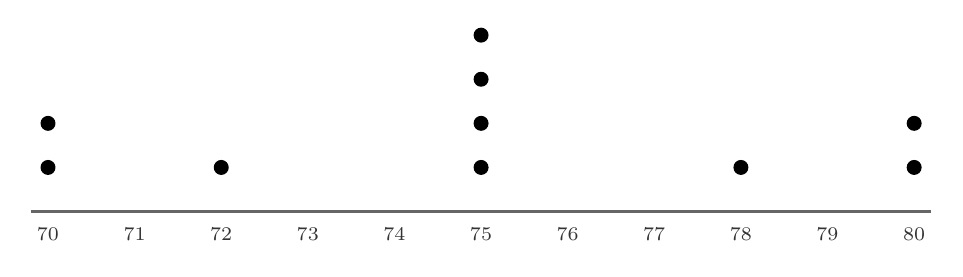
\begin{tikzpicture}[x=1.1cm, y=0.8cm]
    \draw[thick, black!60] (69.8,0) -- (80.2,0);
    \foreach \x in {70,71,72,73,74,75,76,77,78,79,80} {
        \node[below, font=\scriptsize, text=black!80] at (\x,-0.1) {\x};
    }
    \foreach \x/\y in {70/0.7, 70/1.4, 72/0.7, 75/0.7, 75/1.4, 75/2.1, 75/2.8, 78/0.7, 80/0.7, 80/1.4} {
        \filldraw[black] (\x,\y) circle (2.5pt);
    }
\end{tikzpicture}
\end{center}

\item 
\begin{rlist}
    \item Για τη μέση τιμή ισχύει
    \[ \bar{x} = \frac{\sum t_i}{\nu} = \frac{70+70+72+75+75+75+75+78+80+80}{10} = \frac{750}{10} = 75 \]
    
    \item Τοποθετούμε τις παρατηρήσεις σε αύξουσα σειρά και έχουμε
    
    $70,\ 70,\ 72,\ 75,\ 75,\ 75,\ 75,\ 78,\ 80,\ 80$
    
    Επειδή το πλήθος των παρατηρήσεων είναι άρτιο $\nu = 10$, η διάμεσος δίνεται από το ημιάθροισμα των δύο μεσαίων παρατηρήσεων.
    
    Άρα $\delta = \frac{t_5 + t_6}{2} = \frac{75+75}{2} = 75$
\end{rlist}
\end{alist}
\vspace{6mm}
\noindent\rule{\textwidth}{0.4pt}
\vspace{6mm}

